\documentclass{article}

\usepackage[top=0mm,bottom=40mm,right=30mm,left=30mm]{geometry}
\usepackage{fancyhdr}
\usepackage[style=long3col]{glossaries}
\usepackage{hyperref}
\usepackage{graphicx}
\usepackage{caption}
\captionsetup{%
    format=plain,%
    textformat=period,
    justification=RaggedRight,
    singlelinecheck=true,
}%

\makenoidxglossaries
\setlength{\glsdescwidth}{0.8\textwidth}
%\renewcommand*{\glsgroupskip}{}

\newglossaryentry{animal}{
    name = {animal},
    sort = {animal},
    description = {Any living thing that is not a plant (basically)}
}

\usepackage[tikz]{mdframed}
\usepackage{xcolor,comment}
\usepackage{enumerate, multicol}
\newmdenv[backgroundcolor=answerboxcolor]{answerbox}
\colorlet{answerboxcolor}{blue!20}

\fancyhf{}

\title{\uppercase{the} Best Pre \textbf{AND} Post Nutrition for \textsc{Ultimate Frisbee} Athletes}
\author{Aayush Bajaj}
\date{\today}

\begin{document}

\maketitle
\thispagestyle{fancy}
\dotfill

\vspace{0.5cm}
\fbox{
    \centering
\begin{minipage}{0.9\textwidth}
    \begin{flushleft} \large\emph{We are what we repeatedly do, excellence then is not an act, but a habit.} \end{flushleft}
    \begin{flushright}--- Will Durant\end{flushright}
\end{minipage}
}

\hrulefill

\begin{answerbox}
    \section*{Solution}
    To find an optimal solution this time we must appeal to Nature and therefore time. Homo-Sapiens evolved in East Africa 200,000 years ago. From then until 10,000 years ago we have been operating as \textbf{Hunter Gatherers}. As such we have physiologically evolved with specific mechanisms to support these behaviours. Namely, we have the ability to last without food for reasonable periods of time (i.e. not being successful on a hunt), being calorically saturated for longer windows of time (i.e. being successful with gathering). Additionally, considering advances of science with unveiling the structure of muscles we can gain insight into their macro and micro nutrient requirements. Specifically, we require protein after micro-tearing muscle fibres, micro-nutrients such as creatine, potassium and magnesium to enhance performance. Considering these broad factors we can template an optimal diet.

    \begin{multicols}{2}
        \subsection*{Pre Game}
            \begin{enumerate}
                \item Empty Stomach (triggers the hunting reflex)
                    \begin{itemize}
                        \item Note that this relies on adequate micro-nutrient dosing prior to the game (i.e. taking your creatine daily, consuming the multivitamins)
                    \end{itemize}
                \item Light fruits, gives glycogen sustenance whilst not comprising athletic ability
            \end{enumerate}
        \subsection*{Post Game}
            Do not consume a large amount of calories immediately, but rather build momentum with caloric intake over the course of a longer feeding window (i.e. 3 hours). Else the digestive system enters a state of shock, is unable to metabolize correctly and thus cramps ensue. Ensure foods are calorically dense, avoid process foods until after a good base has been consumed: c.f figure 1 for the glycogen effects after a base vs pre-base. 
    \end{multicols}


\end{answerbox}

\begin{minipage}{\textwidth}
    \centering
    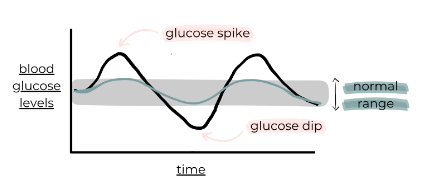
\includegraphics[width=0.4\textwidth]{glycogen.png}
    \captionof{figure}{Glycogen Spikes}
\end{minipage}

\vspace*{-0.5cm}
\printnoidxglossary[style=listdotted]

\begin{thebibliography}{8}
    \bibitem{nh} Yuval Noah Harari, \emph{Sapiens, A Brief History of Humankind}, 2014

\end{thebibliography}


\end{document}
